%%
%% This is file `elsarticle-template-num.tex',
%% generated with the docstrip utility.
%%
%% The original source files were:
%%
%% elsarticle.dtx  (with options: `numtemplate')
%% 
%% Copyright 2007, 2008 Elsevier Ltd.
%% 
%% This file is part of the 'Elsarticle Bundle'.
%% -------------------------------------------
%% 
%% It may be distributed under the conditions of the LaTeX Project Public
%% License, either version 1.2 of this license or (at your option) any
%% later version.  The latest version of this license is in
%%    http://www.latex-project.org/lppl.txt
%% and version 1.2 or later is part of all distributions of LaTeX
%% version 1999/12/01 or later.
%% 
%% The list of all files belonging to the 'Elsarticle Bundle' is
%% given in the file `manifest.txt'.
%% 

%% Template article for Elsevier's document class `elsarticle'
%% with numbered style bibliographic references
%% SP 2008/03/01

%\documentclass[preprint,12pt]{elsarticle}
\documentclass[preprint,10pt]{elsarticle}
%\documentclass[final,3p,times]{elsarticle} 

%% Use the option review to obtain double line spacing
%% \documentclass[authoryear,preprint,review,12pt]{elsarticle}

%% Use the options 1p,twocolumn; 3p; 3p,twocolumn; 5p; or 5p,twocolumn
%% for a journal layout:
%% \documentclass[final,1p,times]{elsarticle}
%% \documentclass[final,1p,times,twocolumn]{elsarticle}
%% \documentclass[final,3p,times]{elsarticle}
%% \documentclass[final,3p,times,twocolumn]{elsarticle}
%% \documentclass[final,5p,times]{elsarticle}
%% \documentclass[final,5p,times,twocolumn]{elsarticle}

%% if you use PostScript figures in your article
%% use the graphics package for simple commands
%\usepackage{graphics}
%\usepackage{float}
\usepackage{subfigure}
%\usepackage{subfig}

\usepackage{color}
%% or use the graphicx package for more complicated commands
\usepackage{graphicx}
%% or use the epsfig package if you prefer to use the old commands
%% \usepackage{epsfig}

%% The amssymb package provides various useful mathematical symbols 
%% The amsthm package provides extended theorem environments
\usepackage{amssymb}
\usepackage{amsmath}
% more math
\usepackage{amsfonts}
\usepackage{amssymb}
\usepackage{amstext}
\usepackage{amsbsy}

\usepackage{mathbbol} % permet d'avoir le vrai symbol pour les reels grace a mathbb
%\usepackage{enumerate} % permet d'utiliser enumerate
%\usepackage{moreverb} % permet d'utiliser verbatimtab : conservation la tabulation
\usepackage{stmaryrd} % permet d'utiliser \llbrackedt et \rrbracket : double crochet
%\usepackage[noabbrev]{cleveref} % permet d'utiliser cref and Cref
%\usepackage{caption} % permet d'utiliser subcaption
%\usepackage{subcaption} % permet d'utiliser subfigure, subtable, etc
%\usepackage[margin=1.in]{geometry}


%% The lineno packages adds line numbers. Start line numbering with
%% \begin{linenumbers}, end it with \end{linenumbers}. Or switch it on
%% for the whole article with \linenumbers.
\usepackage{lineno}

\journal{Journal of Comp. Phys.}
%%%%%%%%%%%%%%%%%%%%%%%%%%%%%%%%%%%%%%%%%%%%%%%%%%%%%%%%%%%%%%%%%%%%
% operators
\renewcommand{\div}{\vec{\nabla}\! \cdot \!}
\newcommand{\grad}{\vec{\nabla}}
% latex shortcuts
\newcommand{\bea}{\begin{eqnarray}}
\newcommand{\eea}{\end{eqnarray}}
\newcommand{\be}{\begin{equation}}
\newcommand{\ee}{\end{equation}}
\newcommand{\bal}{\begin{align}}
\newcommand{\eali}{\end{align}}
\newcommand{\bi}{\begin{itemize}}
\newcommand{\ei}{\end{itemize}}
\newcommand{\ben}{\begin{enumerate}}
\newcommand{\een}{\end{enumerate}}
% DGFEM commands
\newcommand{\jmp}[1]{[\![#1]\!]}                     % jump
\newcommand{\mvl}[1]{\{\!\!\{#1\}\!\!\}}             % mean value
\newcommand{\keff}{\ensuremath{k_{\textit{eff}}}\xspace}
% shortcut for domain notation
\newcommand{\D}{\mathcal{D}}
\newcommand{\J}{\mathcal{J}}
\newcommand{\I}{\mathcal{I}}
% vector shortcuts
\newcommand{\vo}{\vec{\Omega}}
\newcommand{\vr}{\vec{r}}
\newcommand{\vn}{\vec{n}}
\newcommand{\vnk}{\vec{\mathbf{n}}}
\newcommand{\vj}{\vec{J}}
% extra space
\newcommand{\qq}{\quad\quad}
% common reference commands
\newcommand{\eqt}[1]{Eq.~(\ref{#1})}                     % equation
\newcommand{\fig}[1]{Fig.~\ref{#1}}                      % figure
\newcommand{\tbl}[1]{Table~\ref{#1}}                     % table
\newcommand{\sct}[1]{Section~\ref{#1}}                   % section

\newcommand{\ud}{\,\mathrm{d}}
\newcommand{\mt}[1]{\marginpar{ {\tiny #1}}}

\newcommand\bn{\boldsymbol{\nabla}}
\newcommand\bo{\boldsymbol{\Omega}}
\newcommand\br{\mathbf{r}}
\newcommand\la{\left\langle}
\newcommand\ra{\right\rangle}
\newcommand\bs{\boldsymbol}
\newcommand\red{\textcolor{red}}
\newcommand\blue{\textcolor{blue}}
\newcommand\ldb{\{\!\!\{}
\newcommand\rdb{\}\!\!\}}
\newcommand\llb{\llbracket}
\newcommand\rrb{\rrbracket}
\newcommand\mc{\mathcal}
%\newcommand{\tf}{\varphi}
\newcommand{\tf}{b}

\renewcommand{\(}{\left(}
\renewcommand{\)}{\right)}
\renewcommand{\[}{\left[}
\renewcommand{\]}{\right]}

\newcommand{\tcr}[1]{\textcolor{red}{#1}}
%%%%%%%%%%%%%%%%%%%%%%%%%%%%%%%%%%%%%%%%%%%%%%%%%%%%%%%%%%%%%%%%%%%%%
%
%   BEGIN DOCUMENT
%
%%%%%%%%%%%%%%%%%%%%%%%%%%%%%%%%%%%%%%%%%%%%%%%%%%%%%%%%%%%%%%%%%%%%%
\begin{document}

 

%%%%%%%%%%%%%%%%%%%%%%%%%%%%%%%%%%%%%%%%%%%%%%%%%%%%%%%%%%%%%%%%%%%%
\begin{frontmatter}

%% Title, authors and addresses

%% use the tnoteref command within \title for footnotes;
%% use the tnotetext command for theassociated footnote;
%% use the fnref command within \author or \address for footnotes;
%% use the fntext command for theassociated footnote;
%% use the corref command within \author for corresponding author footnotes;
%% use the cortext command for theassociated footnote;
%% use the ead command for the email address,
%% and the form \ead[url] for the home page:
%\title{Title\tnoteref{label1}}
%% \tnotetext[label1]{}
%% \author{Name\corref{cor1}\fnref{label2}}
%% \ead{email address}
%% \ead[url]{home page}
%% \fntext[label2]{}
%% \cortext[cor1]{}
%% \address{Address\fnref{label3}}
%% \fntext[label3]{}

%-------------------------
%-------------------------
%\title{Discontinuous Finite Element Solution for Diffusion Equations on Arbitrary Polygonal Meshes}
\title{Discontinuous Finite Element Solution of the Diffusion Equation on Arbitrary Polygonal Meshes}
%-------------------------
%-------------------------

%% use optional labels to link authors explicitly to addresses:
%% \author[label1,label2]{}
%% \address[label1]{}
%% \address[label2]{}

%-------------------------
\author{Bruno Turcksin \fnref{label1}}
\ead{bruno.turcksin@neo.tamu.edu}

\address[label1]{Department of Nuclear Engineering, Texas A\&M University 
  College Station, TX 77843, USA \fnref{label2}}

\author{Jean C. Ragusa\fnref{label1}\corref{cor1}}
\ead{jean.ragusa@tamu.edu}

\cortext[cor1]{Corresponding author}
%-------------------------

%-------------------------
\begin{abstract}

aaaa

\end{abstract}
%-------------------------

%-------------------------
\begin{keyword}
  Radiation Diffusion \sep
	Arbitrary Polygonal Grids \sep
  Piecewise Linear Discontinuous \sep
  Adaptive Mesh Refinement\sep
  Radiation transport \sep
  Discontinuous Finite Element \, .
\end{keyword}
%-------------------------

\end{frontmatter}

%%%%%%%%%%%%%%%%%%%%%%%%%%%%%%%%%%%%%%%%%%%%%%%%%%%%%%%%%%%%%%%%%%%%

\linenumbers

%%%%%%%%%%%%%%%%%%%%%%%%%%%%%%%%%%%%%%%%%%%%%%%%%%%%%%%%%%%%%%%%%%%%%%%%%%%%%%%%%%%%%%%%%%%%%%%%%%%%
%%%%%%%%%%%%%%%%%%%%%%%%%%%%%%%%%%%%%%%%%%%%%%%%%%%%%%%%%%%%%%%%%%%%%%%%%%%%%%%%%%%%%%%%%%%%%%%%%%%%
\section{Introduction} \label{sec:intro}
%%%%%%%%%%%%%%%%%%%%%%%%%%%%%%%%%%%%%%%%%%%%%%%%%%%%%%%%%%%%%%%%%%%%%%%%%%%%%%%%%%%%%%%%%%%%%%%%%%%%
%%%%%%%%%%%%%%%%%%%%%%%%%%%%%%%%%%%%%%%%%%%%%%%%%%%%%%%%%%%%%%%%%%%%%%%%%%%%%%%%%%%%%%%%%%%%%%%%%%%%

\red{Make sure the following is expressed somewhere:\\
In this
research, we focus on using PWLD to discretize the diffusion equation. The
PWLD discretization employs discontinuous finite elements and has been used to
discretize the transport equation. Using it to discretize the diffusion
equation is an important step in order to create a Diffusion Synthetic
Acceleration scheme \cite{Adams2002,Wang2010}.
}

This paper deals with a discontinuous finite element spatial discretizations of the radiation 
diffusion equation on arbitrary polygonal grids, with and without adaptive mesh refinement. 
Radiation diffusion is an asymptotic limit of the radiation transport equation and can be 
written in the following form:
\begin{equation} \label{eq:radiation_diffusion}
- \div  D(\vr) \grad E(\vr) + \sigma_a(\vr) E(\vr) = Q(\vr) ,
\end{equation}
where $E$ is the radiation energy intensity, $D$ is a diffusion coefficient, $\sigma_a$ is 
an opacity coefficient, and $Q$ is the source.

Several spatial discretizations have been proposed to solve \eqt{eq:radiation_diffusion} on
arbitrary polygons (2D) and polyhedra (3D) \cite{Wachspress,Kuznetsov2004,Palmer2005,Brezzi2005,
LipnikovShashkovSvyatskiy2006,BaileyAdams2008}. We review them below.
%
Wachspress \cite{Wachspress} developed a family of rational polynomial functions that can be employed
as basis functions in a finite element method on polygonal/polyhedral grids. This yields
symmetric positive-definite (SPD) matrices but (i) the finite element integrals must be carried out 
numerically and (ii) the Jacobian of the transformation becomes zero on degenerate cells 
(such as the ones shown on \fig{fig:amr_schematics}). 
%
%Morel et al. \cite{MorelDendyHallWhite1992} introduced a cell-centered finite volume scheme 
%for arbitrary quadrilateral meshes. Their scheme was second-order accurate and yielded back a 
%standard five-point stencil on orthogonal grids, but the diffusion operator was asymmetric 
%and cell-edge unknowns were added in addition to cell-center unknowns.
%%
Palmer \cite{Palmer2005,PalmerLLNL} proposed a node-based finite volume method 
that enforces particle balance over dual cells, where a dual cell is defined as 
the union of all corners surrounding a given vertex $p$ and where  a corner 
is a quadrilateral defined by vertex $p$, the cell center, and the midpoint
of the edges that contain vertex $p$. On a triangular grid, Palmer's scheme is equivalent 
to linear continuous finite elements with ``mass-matrix lumping''. The method is 
second-order accurate but the discretization of the diffusion equation using Palmer's method 
does not result in SPD matrices.
%
Mimetic finite difference methods create discrete analog of vector and tensor
calculus in order to accurately approximate the original differential operators;
see, e.g., \cite{HymanMorelShashkovSteinberg2002}.
Mimetic methods preserve important properties of the differential operators such 
as symmetry, positivity, monotonicity, asymptotic limits, and identities pertaining 
to tensor and vector calculus. Mimetic methods can also be viewed as mixed hybrid 
finite element formulations with specific spatial quadratures.  
In addition to quadrilateral and hexahedral meshes (see, e.g., 
\cite{MorelRobertsShashkov1998,MorelHallShashkov2001}, mimetic finite difference 
methods have recently been applied to the diffusion equation on arbitrary polygonal 
grids \cite{Kuznetsov2004,Brezzi2005,LipnikovShashkovSvyatskiy2006,LipnikovShashkov2010}.
%conformal quadrilateral \cite{HymanShashkovSteinberg1997, ShashkovSteinberg1996,MorelRobertsShashkov1998} 
%and hexahedral \cite{MorelHallShashkov2001} grids, locally refined grids \cite{LipnikovMorelShashkov2004}, and
%arbitrary polygonal grids \cote{Kuznetsov2004,Brezzi2005,LipnikovShashkovSvyatskiy2006,LipnikovShashkov2010}.
%
%, scalar and vector inner products, such as: ,
%conservation laws, symmetry preservation, solution positivity and
%monotonicity, and asymptotic limits (e.g., diffusion limit), on polygonal and
%polyhedral meshes. The most important part of MFD is the definition of a scalar
%product which satisfies stability and consistency some conditions
%\cite{Brezzi2005}. However, this scalar product is not unique and therefore,
%multiple MFD methods exists. MFD is efficient even on concave polygons
%\cite{Kuznetsov2004}. MFD methods are related to mixed finite elements.
%
Bailey et al. \cite{BaileyAdams2008} recently employed piecewise linear basis
functions to solve a diffusion equation using a Galerkin finite element technique on 
arbitrary polygonal and polyhedral grids. Their goal was to devise a {\em continuous} finite 
element discretization that does not necessitate numerical integration, yields an SPD matrix, 
is second-order accurate, and handles arbitrary polygonal/polyhedral grids (including 
grids with degenerate cells). The approach they followed is a standard Galerkin weak 
formulation for continuous finite elements, with piecewise linear basis functions 
defined on subcells (which they called ``sides'') of arbitrary polygons/polyhedrons.

In this paper, we are interested in solving a diffusion equation on arbitrary polygonal
grids using a {\em discontinuous} finite element discretization. We employ the
Symmetric Interior Penalty (SIP) technique \cite{IPRefs}, developed for the discretization
of elliptic equations using discontinuous Galerkin techniques. For basis functions,
we use the piecewise linear functions of \cite{BaileyAdams2008}.
The motivations are three-fold: 
\begin{enumerate}
\item we wish to assess the performance of the discontinuous finite elements for 
the discretization of the diffusion equation on polygonal meshes;
\item a diffusion equation often serves as a synthetic accelerator or as a
preconditioner for iterative solution techniques of the particle transport equation
\cite{AdamsLarsen2002}. A discontinuous finite element technique is often employ
in the discretization of the transport equation for unstructured and 
polygonal/polyhedral grids \cite{MorelWarsaWareing,PWLD,CFEM-PWDL-Warsa,WangRagusa}.
Employing the same    
\item 
\end{enumerate}
The motivations for our work / In this work, we wish to assess ... In addition,
a diffusion equation often serves as a synthetic accelerator or as a
preconditioner \cite{AdamsLarsen2002} for iterative solution techniques of the 
radiation transport equation.
% , where a discontinuous finite element technique is often preferred
% in the discretization of the transport equation for unstructured and 
% polygonal/polyhedral grids \cite{MorelWarsaWareing,PWLD,CFEM-PWDL-Warsa,WangRagusa}.

The remainder of the paper is as follows. In \sct{sec:poly}, we discuss
the use of polygonal meshes, recall the definition of the piecewise linear
basis functions for arbitrary polygons, and point out how polygonal grids
can be utilized in handling local mesh refinement (as in adaptive mesh refinement 
approaches). The Symmetric Interior Penalty technique is reviewed in \sct{sec:ip}.
The resulting linear system will be solved using an Algebraic Multi-Grid (AMG) approach.
Results are presented in \sct{sec:results}; all of the test cases presented
are borrowed from the literature on (1) finite differences applied to the
diffusion equation on non 

%%%%%%%%%%%%%%%%%%%%%%%%%%%%%%%%%%%%%%%%%%%%%%%%%%%%%%%%%%%%%%%%%%%%%%%%%%%%%%%%%%%%%%%%%%%%%%%%%%%%
%%%%%%%%%%%%%%%%%%%%%%%%%%%%%%%%%%%%%%%%%%%%%%%%%%%%%%%%%%%%%%%%%%%%%%%%%%%%%%%%%%%%%%%%%%%%%%%%%%%%
\section{Polygonal Grids and Piecewise Linear Basis Functions} \label{sec:poly}
%%%%%%%%%%%%%%%%%%%%%%%%%%%%%%%%%%%%%%%%%%%%%%%%%%%%%%%%%%%%%%%%%%%%%%%%%%%%%%%%%%%%%%%%%%%%%%%%%%%%
%%%%%%%%%%%%%%%%%%%%%%%%%%%%%%%%%%%%%%%%%%%%%%%%%%%%%%%%%%%%%%%%%%%%%%%%%%%%%%%%%%%%%%%%%%%%%%%%%%%%
%-----------------------------------------------------------
\subsection{Polygonal Meshes and their Application to Adaptive Mesh Refinement}
%-----------------------------------------------------------

Polygonal cells are an alternative to standard (triangles/quads) mesh partitioning.
Mesh generation using polygons (polyhedra in 3D) is an active area of research.
Some meshing tools, such as MSTK \cite{mstk} and the Computational Geometry Algorithms 
Library \cite{cgal}, may be employed to generate/process polygonal meshes.  
Several CFD codes (Fluent, StarCCM, OpenFoam) offer polygonal mesh and solver capabilities. 

The rationale for polygonal/polyhedral cells is as follows. 
While quadrilaterals (hexahedra in 3D) can be seen as the standard cell shapes for logically 
structured meshes, they may be difficult to employ in complex geometries. For unstructured meshes,
triangles (tetrahedra in 3D) are the typical building blocks and are employed in 
numerous automated meshing algorithms, but are not well-suited for boundary layers, 
for instance, and may require higher cell counts than quad/hex meshes for a similar
resolution.  The following features of polygonal cells are noteworthy:
\begin{itemize}
  \item Optimal partition of the domain, minimizing the boundary/interior ratio;
  \item Reduction in the number of unknowns for equivalent accuracy (akin to
	hex meshes over tet meshes);
	\item The notion of transition elements is included by default in arbitrary grids composed of
	polygons/polyhedra. Therefore, such a grid can easily be split by cut planes, for 
	instance. 
  \item The notion of ``hanging nodes'' for locally refined /adapted meshed is no longer needed.
	For example, \fig{fig:amr1} shows two quadrilateral elements before local refinement; on
	\fig{fig:amr2}, one of the two cells has been refined. The un-refined cell is now viewed as a
	pentagon.
\end{itemize}

\begin{figure}[!hbtp]
\centering
%\vspace{40mm}
%\hspace{-55mm}
\subfigure[before local refinement]{
\includegraphics[scale=0.55]{amr1.png}
\label{fig:amr1}
}
%\hspace{45mm}
\subfigure[after local refinement]{
\includegraphics[scale=0.55]{amr2.png}
\label{fig:amr2}
}
\caption{Local mesh refinement leads to pentagonal cell}
\label{fig:amr}
\end{figure}


%-----------------------------------------------------------
\subsection{Piecewise Linear Basis Functions on Arbitrary Polygons}
%-----------------------------------------------------------

Consider a polygonal cell with $N_V$ vertices, $(x_i,y_i)$. The polygon needs not 
to be convex. In order to describe the piecewise linear basis functions
for such a cell, we introduce a cell ``center'', denoted hereafter 
by $c=(x_c,y_c)$, with $x_c =\sum_{i=1}^{N_V} \alpha_{i} x_i$
and  $y_c = \sum_{i=1}^{N_V} \alpha_{i} y_i$. We require that
$\sum_{i=1}^{N_V} \alpha_{i} = 1$. Point $c$ is a weighted average
of the polygon's vertices. Often, one chooses $\alpha_i = 1 / N_V$.
With the introduction of the cell center, the polygon can be viewed as
$N_V$ triangular subcells, each triangle being composed of two
successive vertices and the cell center.
The $N_V$ piecewise linear basis functions are given by:
%
\begin{equation}
  b_j(\br) = t_j(\br) + \alpha_{j} t_c(\br) , \qquad j=1,\ldots,N_V ,
\end{equation}
%
where $t_j(\br)$ is the standard linear function defined on the two
triangular subcells formed by (i) vertex $j$, vertex $j-1$ and the cell center $c$,
and (ii) vertex $j$, vertex $j+1$ and the cell center $c$.
$t_j$ is equal to one at the $j^{th}$ vertex and to zero all other vertices,
as well as at the cell center.
$t_c(\br)$ is a function associated with the cell center and is equal to one 
at the cell center  and to zero at all of the polygon vertices.
%
We stress that this does not lead to a standard continuous finite element
representation within a polygon that is cut into $N_V$
triangular subcells; in such a case, the number of basis functions
would be $N_V+1$ (for the $N_V$ vertices and the cell center). In the
piecewise linear representation, the unknowns are only located at the cell 
vertices and the cell center point is only used to define the basis functions.
\fig{fig:pentagons} presents two simple examples of polygonal cells: a 
pentagon and a degenerated pentagon, the later is typically obtained
during local mesh adaptation (see also \fig{fig:amr2}).
The isolines of the piecewise linear basis functions for vertex $D$ and
$E$ are graphed in \fig{fig:pwl_pentagon} for the regular pentagon
and in \fig{fig:pwl_degen_pentagon} for the degenerate pentagon as an example.
%
\begin{figure}[!hbtp]
\centering
\includegraphics[scale=0.77]{pentagons.png}
\label{fig:pentagons}
\caption{Non-degenerate and degenerate pentagonal cells}
\end{figure}
%
%
\begin{figure}[!hbtp]
\centering
\subfigure[Basis function for Point D]{
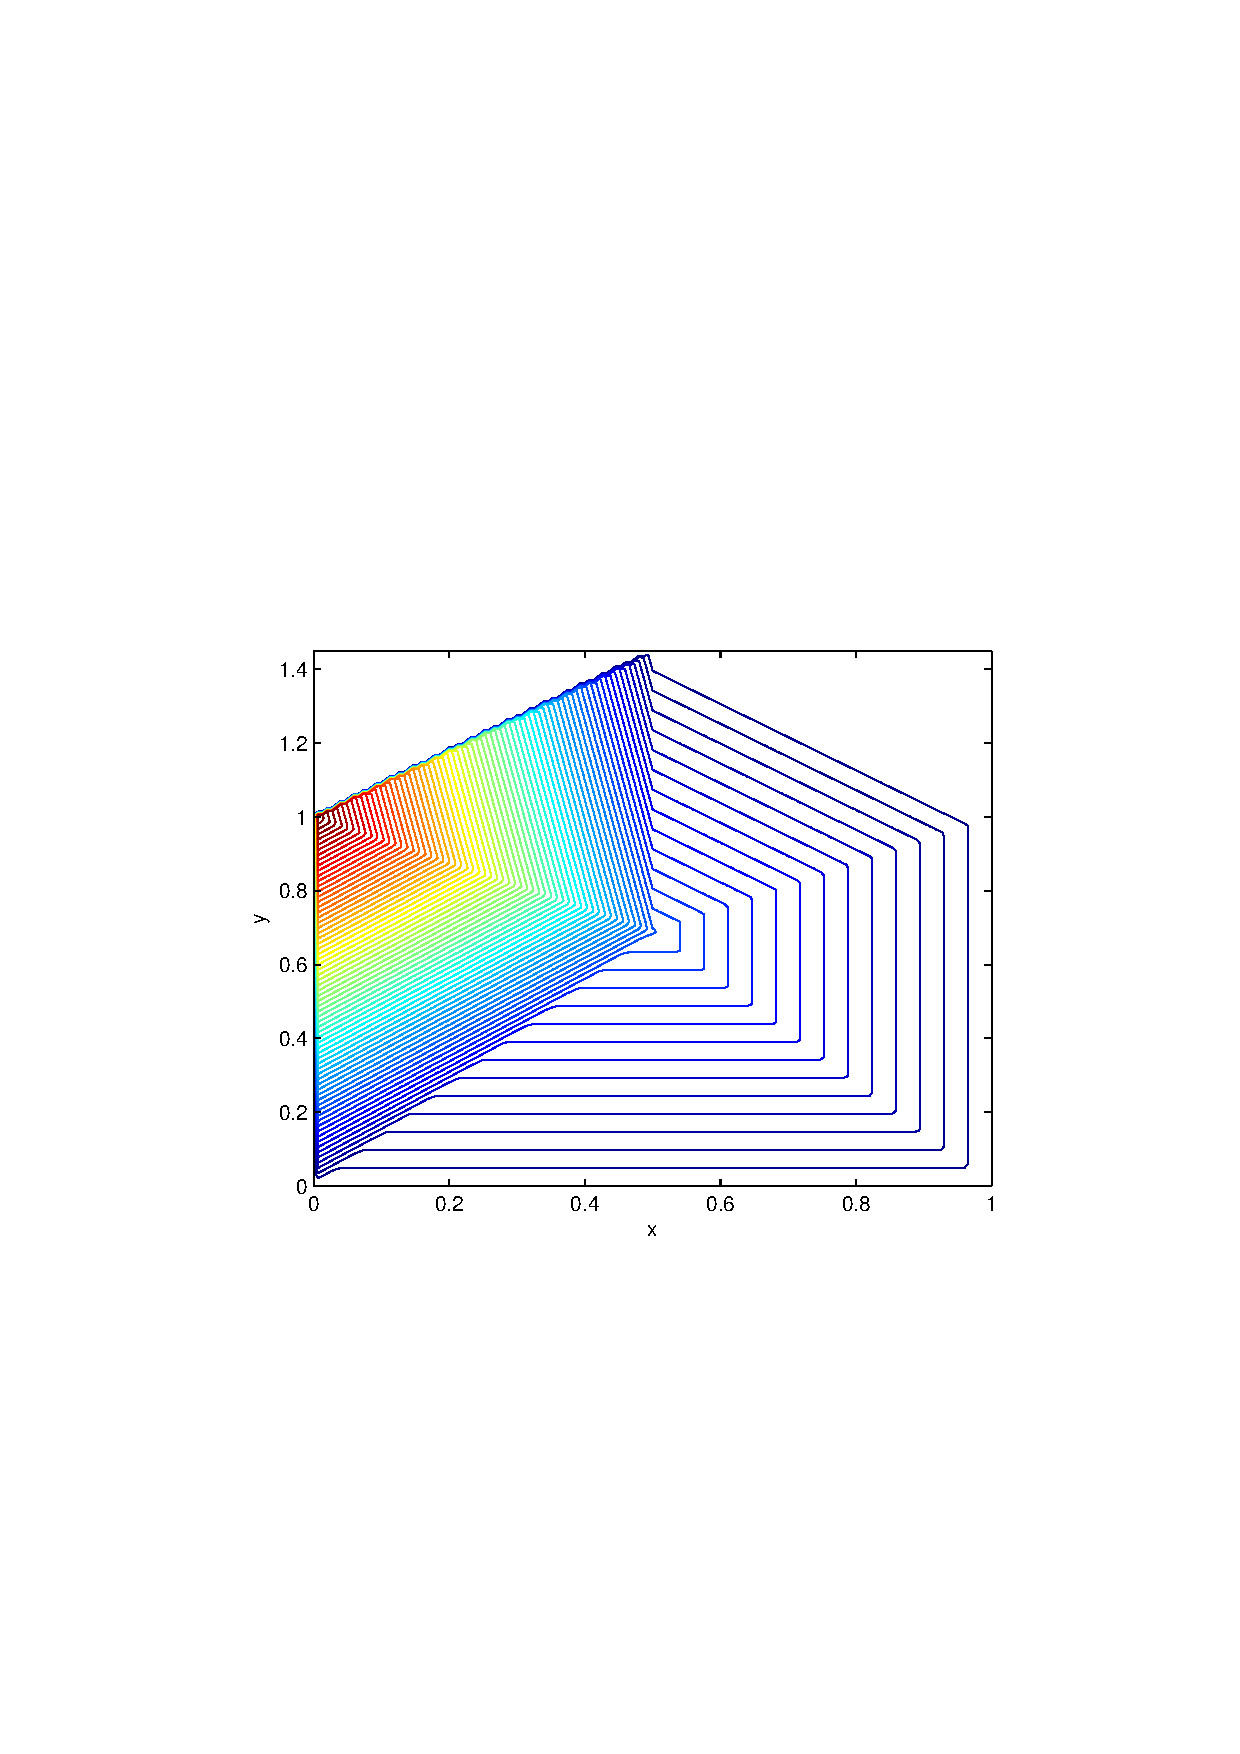
\includegraphics[scale=0.33]{PWL_D.png}
\label{fig:pwl_pentagonD}
}
\subfigure[Basis function for Point E]{
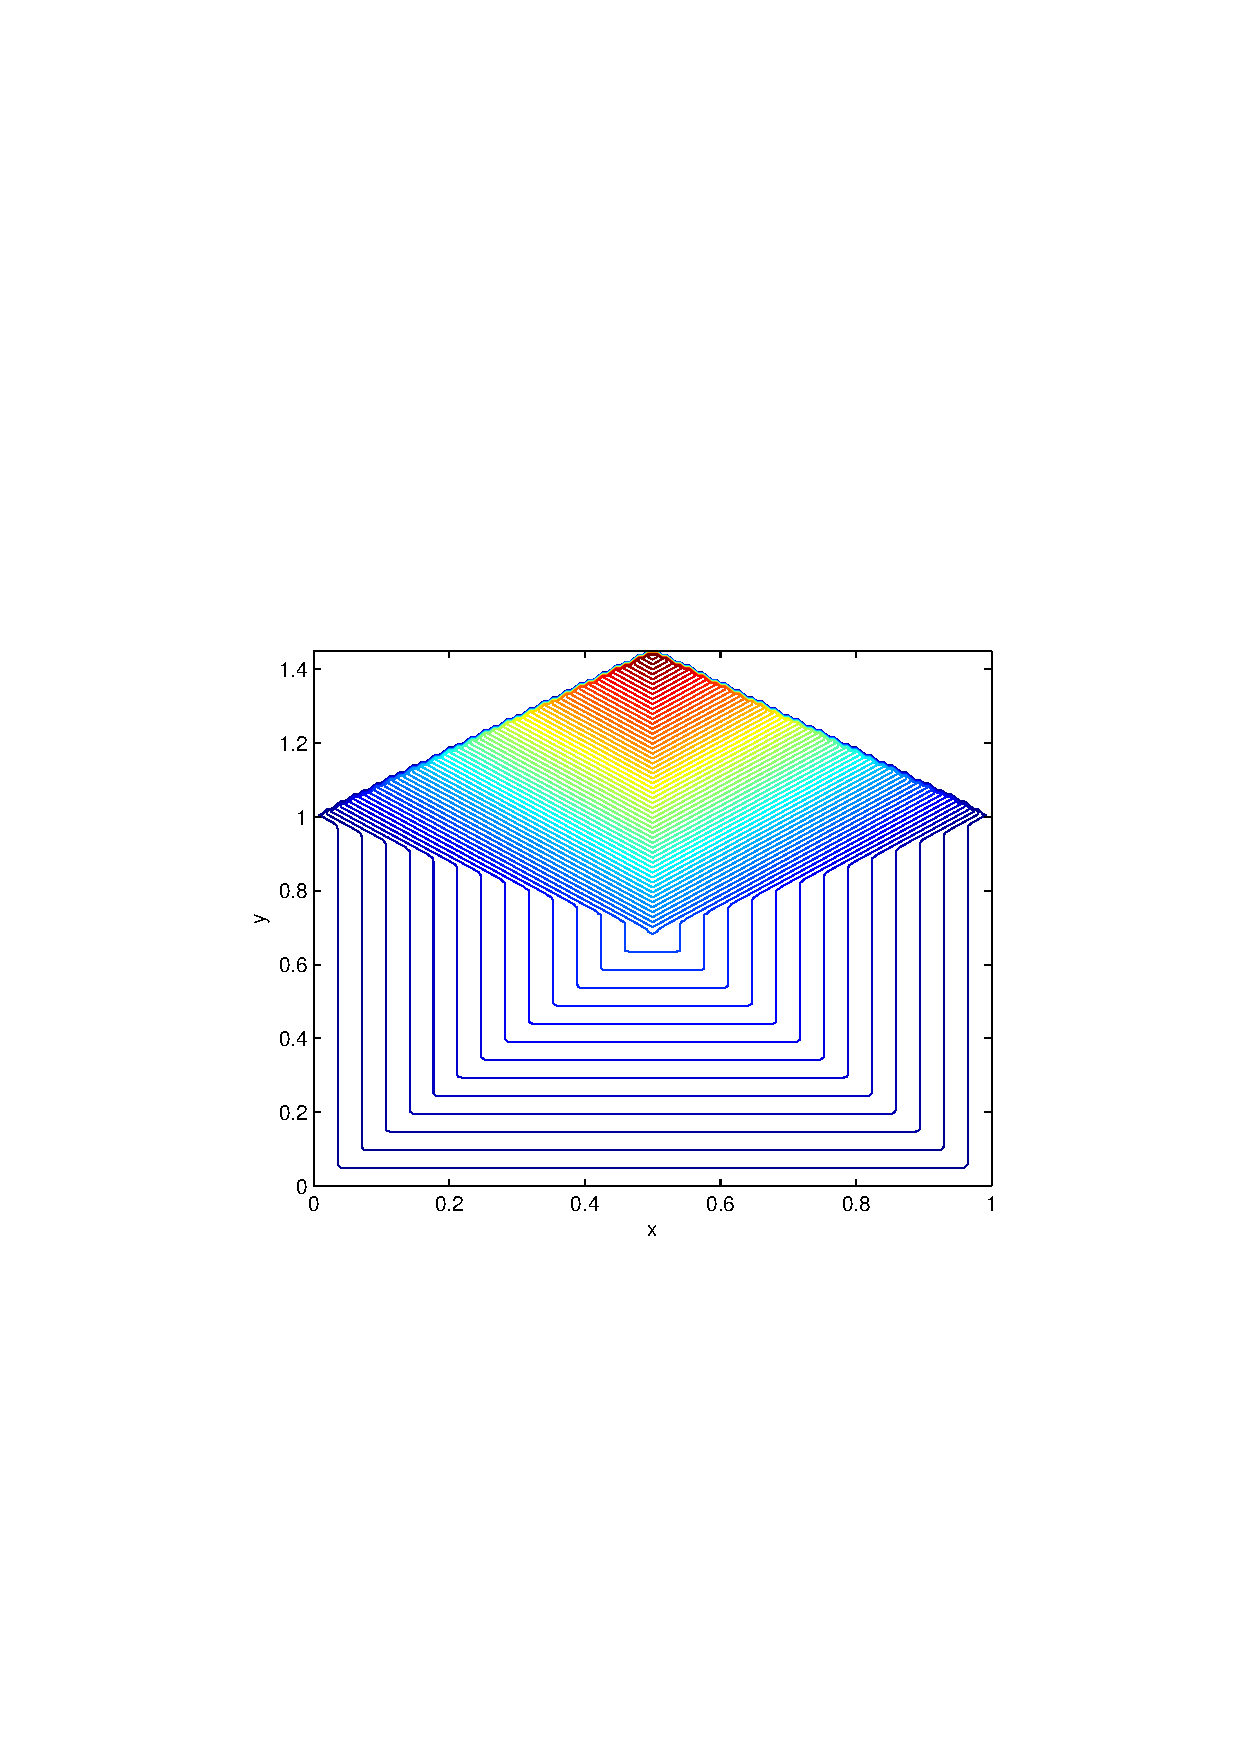
\includegraphics[scale=0.33]{PWL_E.png}
\label{fig:pwl_pentagonE}
}
\caption{PWL basis functions for a non-degenerate pentagon}
\label{fig:pwl_pentagon}
\end{figure}
%
\begin{figure}[!hbtp]
\centering
\subfigure[Basis function for Point D]{
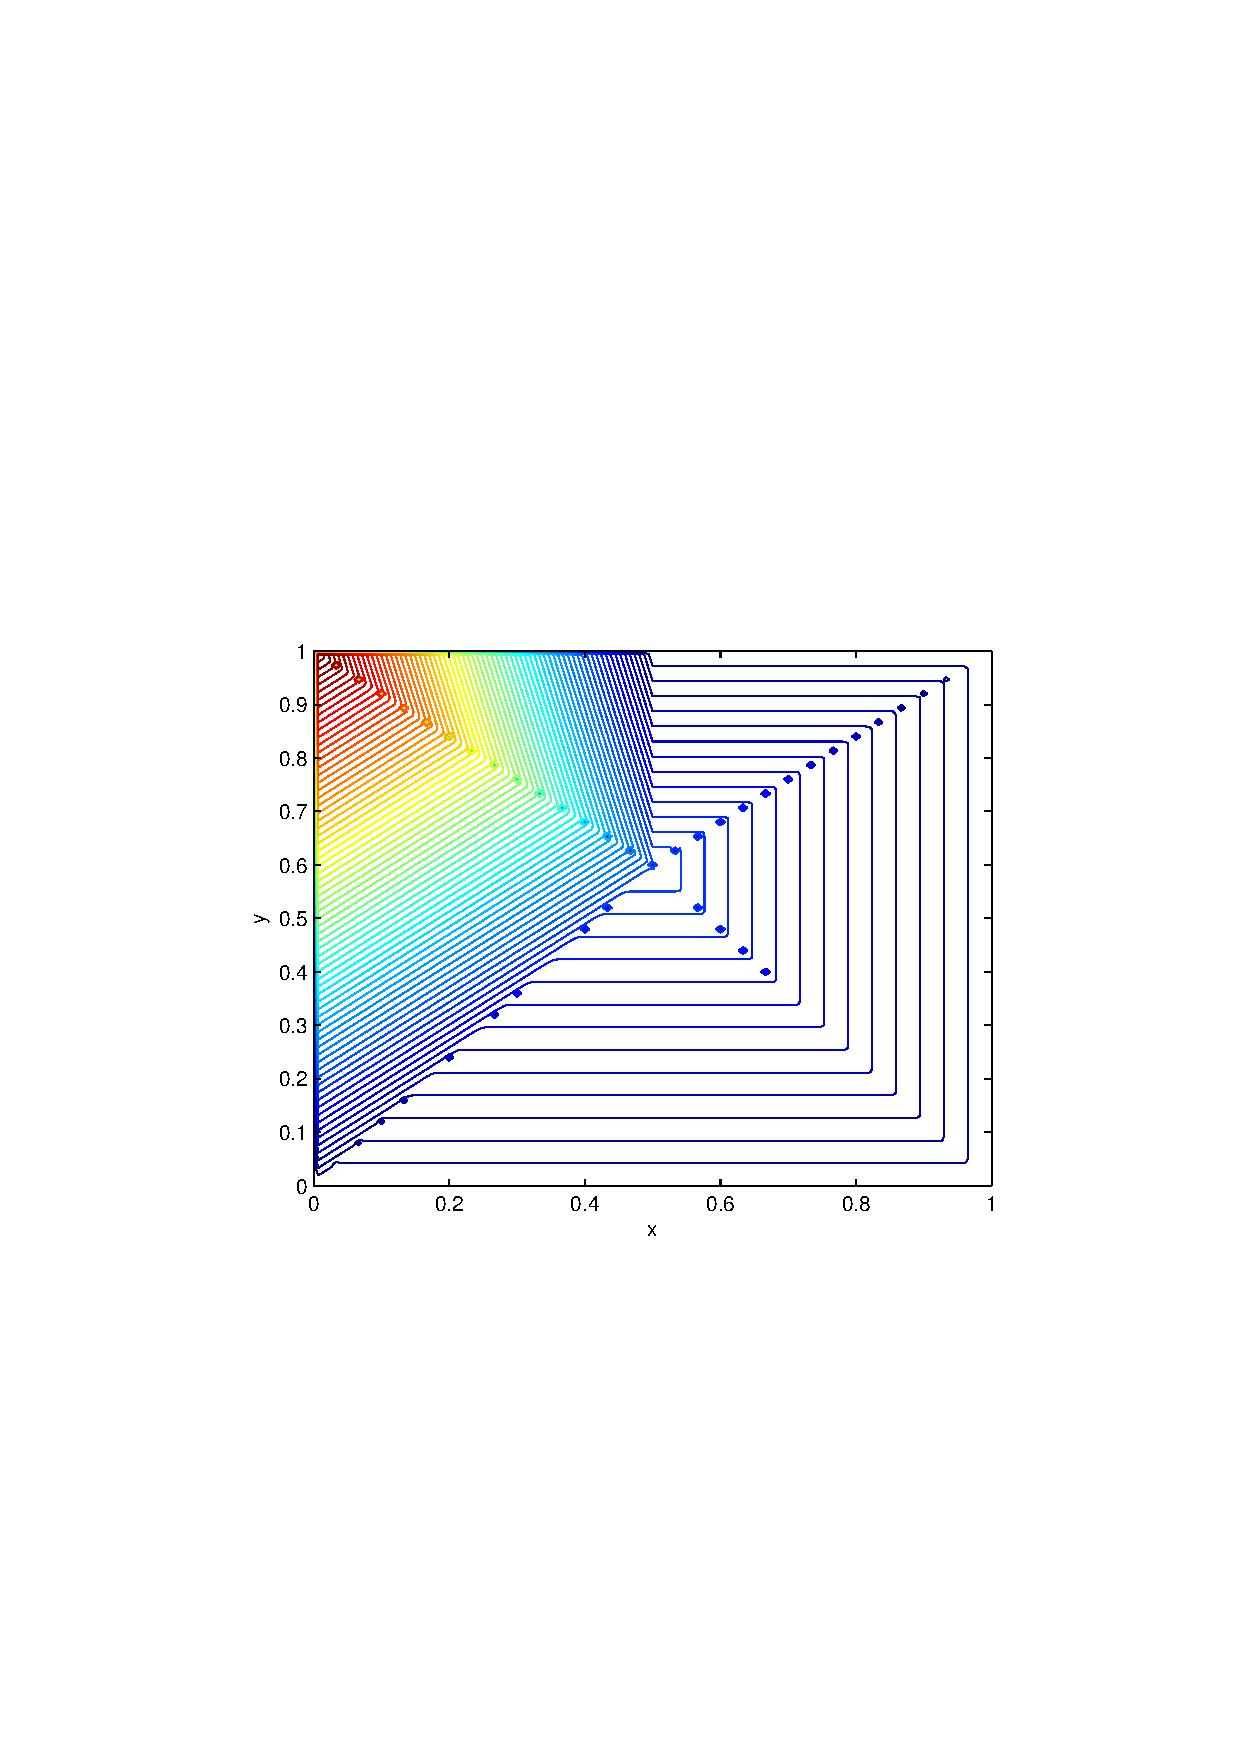
\includegraphics[scale=0.33]{PWL_D_flat.png}
\label{fig:pwl_degen_pentagonD}
}
\subfigure[Basis function for Point E]{
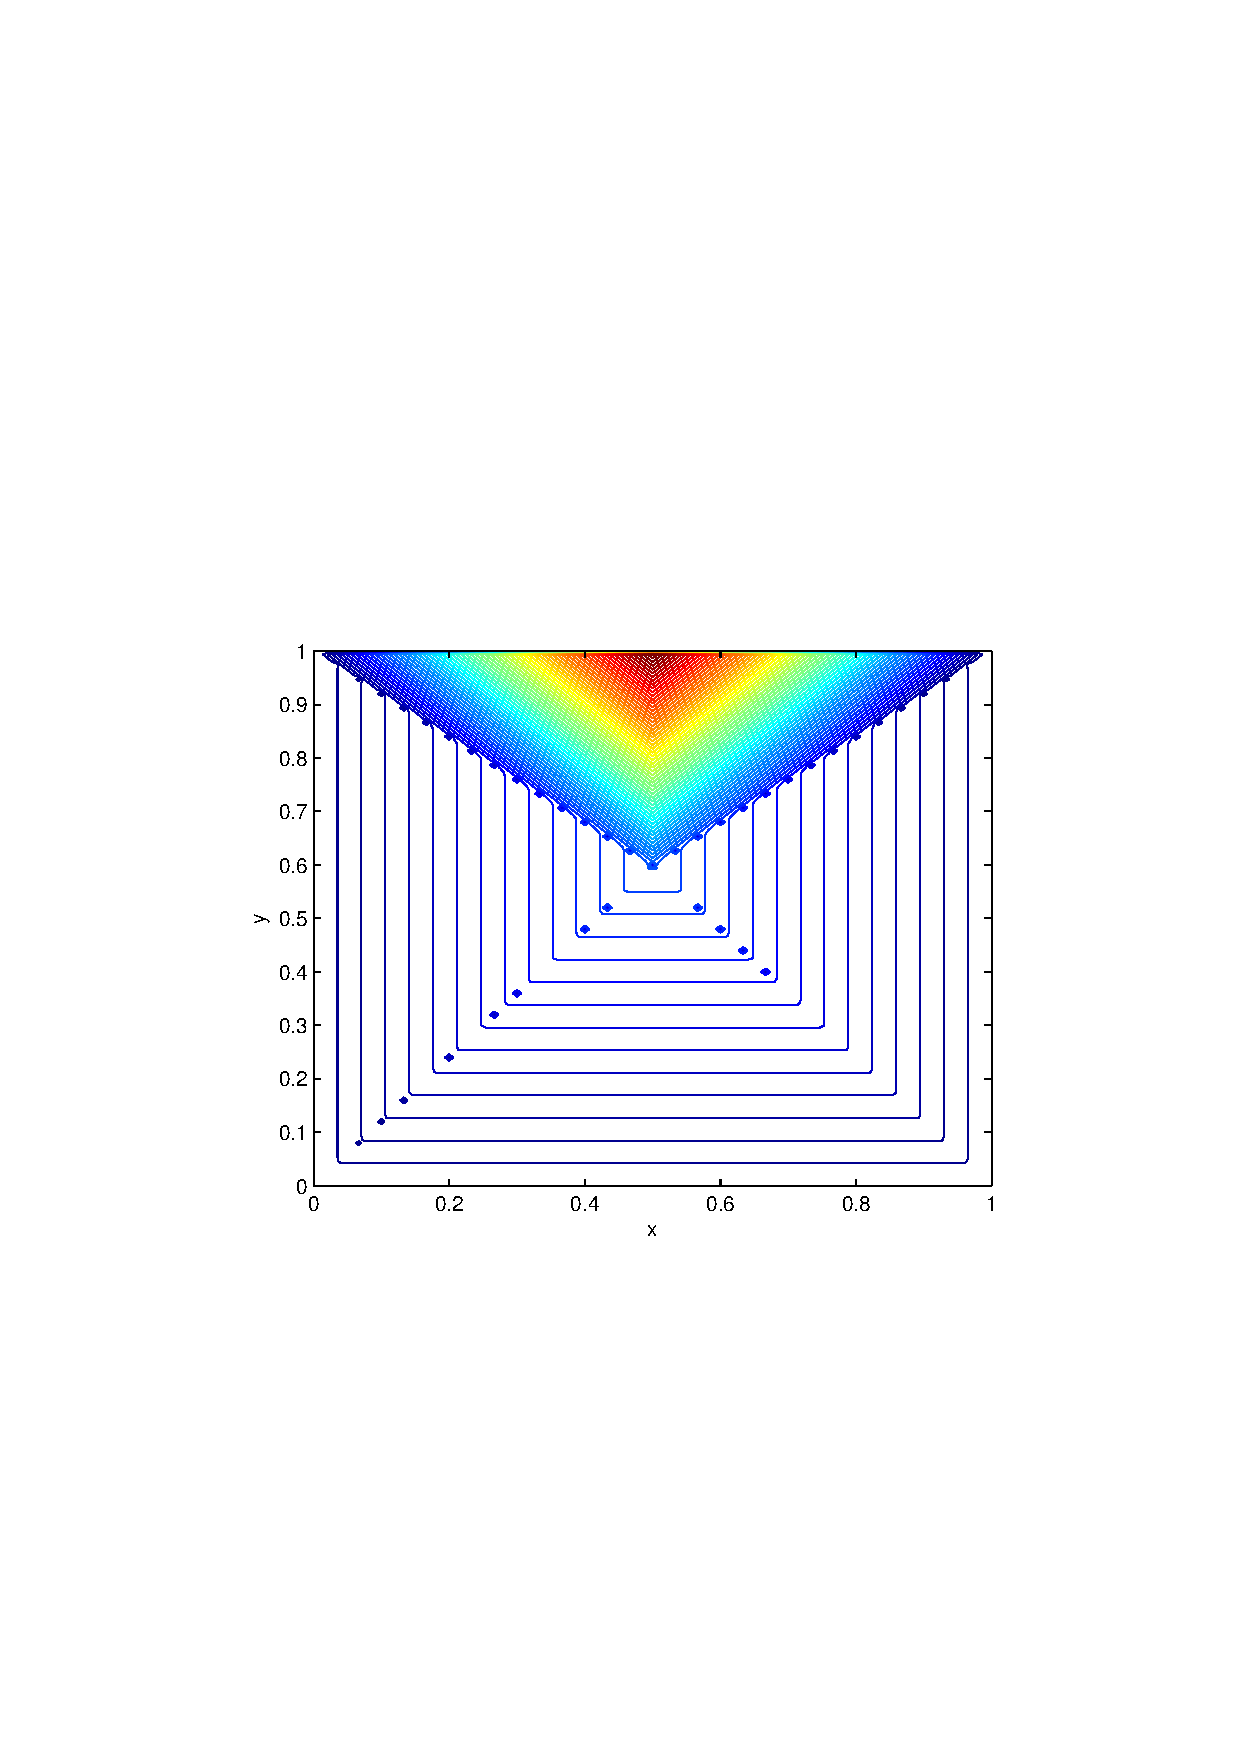
\includegraphics[scale=0.33]{PWL_E_flat.png}
\label{fig:pwl_degen_pentagonE}
}
\caption{PWL basis functions for a degenerate pentagon}
\label{fig:pwl_degen_pentagon}
\end{figure}



%%%%%%%%%%%%%%%%%%%%%%%%%%%%%%%%%%%%%%%%%%%%%%%%%%%%%%%%%%%%%%%%%%%%%%%%%%%%%%%%%%%%%%%%%%%%%%%%%%%%
%%%%%%%%%%%%%%%%%%%%%%%%%%%%%%%%%%%%%%%%%%%%%%%%%%%%%%%%%%%%%%%%%%%%%%%%%%%%%%%%%%%%%%%%%%%%%%%%%%%%
\section{Finite Element Formulation} \label{sec:ip}
%%%%%%%%%%%%%%%%%%%%%%%%%%%%%%%%%%%%%%%%%%%%%%%%%%%%%%%%%%%%%%%%%%%%%%%%%%%%%%%%%%%%%%%%%%%%%%%%%%%%
%%%%%%%%%%%%%%%%%%%%%%%%%%%%%%%%%%%%%%%%%%%%%%%%%%%%%%%%%%%%%%%%%%%%%%%%%%%%%%%%%%%%%%%%%%%%%%%%%%%%

In this Section, we present the discontinuous Galerkin finite element technique employed here to
discretize the radiation diffusion equation on arbitrary polygonal grids. Many variants of such
methods exist for diffusion problems (depending on the choice of stabilization terms, whether 
the diffusion equation is expressed in its mixed form, \ldots). We refer the Readers to the review
papers \cite{unification,brezzi etc} for additional details. Here, we employ the Symmetric
Interior Penalty (SIP) method which we have found to be robust in our test cases and relatively simple 
to implement.
%Even though discontinuous Galerkin methods are commonly used in the particle and radiation transport communities, 
The general idea of interior penalty methods can be traced back to \cite{lions1968}, where the Dirichlet
boundary conditions to the model problem $\{-\dvi \grad E = Q\right$ in domain $\Omega$, $E=E^d$ on 
the boundary $\partial \Omega\}$ have been enforced via a penalty method, thereby modifying the 
boundary condition to read $E+\frac{1}{\mu}\partial_n E = E^d$ with $\mu\gg 1$. Later, 
Nitsche \cite{nitsche1971} proposed a consistent formulation for the enforcement of the 
Dirichlet boundary condition with a penalty term, leading to the weak formulation:
\begin{equation}
\label{eq:penalty_nitsche}
\int_{\Omega} \grad E \cdot \grad \tf
- \int_{\partial\Omega} \partial_n E \tf  
- \int_{\partial\Omega} \partial_n \tf E 
+ \int_{\partial\Omega} \mu(E-E^d) \tf 
=
\int_{\Omega} Q \tf 
- \int_{\partial\Omega} E^d \partial_n \tf ,
\end{equation}
with $\tf$ a finite element basis function and $\mu=\alpha/h$, where $h$ denotes 
the mesh size and $\alpha>1$ is a constant.

This idea, extended to all cell edges (not only cells with edges on the boundary), leads
to the interior penalty methods for discontinuous finite elements. We introduce a partition
of $\bigcup\nolimits_{K\in \mathbb{T}_{h}}K=\Omega$ of the domain $\Omega$ (and assume
that the boundary of the domain, $\partial \Omega$, consists of straight edges only). The 
set of interior and boundary edges is denoted by $\mathcal{E}_h^i$ and $\mathcal{E}_h^{\partial\Omega}$,
respectively.  Then, the SIP weak form is given by
\begin{equation}
\label{eq:penalty_nitsche}
\int_{\Omega} \grad E \cdot \grad \tf
- \int_{\partial\Omega} \mvl{\partial_n E} \jmp{\tf}  
- \int_{\partial\Omega} \jmp{\partial_n \tf} \mvl{E} 
+ \int_{\partial\Omega} \mu(E-E^d) \tf 
=
\int_{\Omega} Q \tf 
- \int_{\partial\Omega} E^d \partial_n \tf ,
\end{equation}

% Obviously, the domain boundary is the  $\partial \Omega = \mathcal{E}_h^{\partial\Omega,D}\cup \mathcal{E}_h^{\partial\Omega,N} \cup \mathcal{E}_h^{\partial\Omega,R}$.
 
%-----------------------------------------------------------
\subsection{SIP}
%-----------------------------------------------------------

The discretization of the diffusion equation using discontinuous finite
elements is not as straightforward as it is when using continuous finite
elements. To discretize the diffusion equation with discontinuous finite elements, 
we apply the interior penalty method \cite{Kanschat2007}:
\begin{equation}
  -\bn D \bn \phi + \Sigma_a \phi = Q_0\ \textrm{ for } \br \in \mc{D},
\end{equation}
\begin{equation}
  \frac{1}{4}\phi - \frac{1}{2} D \partial_n \phi =0\ \textrm{ for } \br \in
  \partial \mc{D}^d,
\end{equation}
and
\begin{equation}
  -D \partial_n \phi = J^{inc}\ \textrm{ for } \br \in \partial \mc{D}^n,
\end{equation}
where $D$ is the diffusion coefficient, $\phi$ is the scalar flux, $\Sigma_a$
is the absorption cross section, $Q_0$ is a volumetric source, $J^{inc}$ is an
incoming current, $\mc{D}$ is the domain, $\partial \mc{D}^d$ is the boundary 
where Dirichlet conditions are applied, and $\partial \mc{D}^n$ is the boundary 
where Neumann conditions are applied.\\ 
After symmetrization, we get the SPD equation:
\begin{equation}
  a(\tilde{\phi},b) = l(b),
\end{equation}
where:
\begin{equation}
  \begin{split}
    a (\tilde{\phi},b) =& \(\Sigma_a \tilde{\phi},b\)_{\mc{D}} + 
    \(D\bn\tilde{\phi},\bn b\)_{\mc{D}} +
    (\kappa_e\ldb\tilde{\phi}\rdb,\ldb b \rdb)_{E_h^i}\\
    &+ \(\ldb\tilde{\phi}\rdb,\llb D\partial_n b \rrb\)_{E_h^i}+ \(\llb D
    \partial_n \tilde{\phi}\rrb,\ldb b \rdb\)_{E_h^i}\\
    &+ \(\kappa_e \tilde{\phi}, b\)_{\partial \mc{D}^d}
    -\frac{1}{2}\(\tilde{\phi},D\partial_n b\)_{\partial \mc{D}^d}
    -\frac{1}{2}\(D\partial_n\tilde{\phi},b\)_{\partial \mc{D}^d}
  \end{split}
\end{equation}
and:
\begin{equation}
  l(b) = (Q_0,b)_{\mc{D}} + (J^{inc},b)_{\partial
  \mc{D}^r},
\end{equation}
with $\tilde{\phi}=(\phi_1 b_1,\hdots, \phi_N b_N)^T$, $b = (b_1,\hdots,b_N)$,
$b_i \in W_{\mc{D}}^h$ $\forall i \in (1,\hdots,N)$,
the mesh $\mc{T}_h$ is used to discretize $\mc{D}$ into non-overlapping linear
elements $K$, such that the union of the elements fully covers $\mc{D}$. The
finite dimensional polynomial space is $W_{\mc{D}}^h = \{f \in L^2(\mc{D});
f|_K \in V_p(K), \forall K \in \mc{T}_h$\}, where $V_p(K)$ is the space of
polynomials of degree up to $p$ on element $K$; the set of interior is $E_h^i
= \cup _{K_1,K_2\in \mc{T}_h}(\partial K_1 \cap \partial K_2)$. We also
define:
\begin{align}
  \ldb \phi \rdb &= \phi^+ - \phi^-,\\
  \llb \phi \rrb &=  \frac{\phi^++\phi^-}{2},
\end{align}
with $\phi^{\pm} = \lim_{s\rightarrow 0^{\pm}} \phi(\br+s \bs{n}_e)$, where
$\bs{n}_e$ is the normal unit vector associated with an edge $e$. On the boundary, 
the normal vector has to be oriented outward whereas the orientation on an
interior edge is arbitrary.\\
The penalty parameter $\kappa_e$ is given:
\begin{equation}
  \kappa_e = \left\{
    \begin{aligned}
      &\frac{c(p^+)}{2}\frac{D^+}{h_{\bot}^+}+\frac{c(p^-)}{2}
      \frac{D^-}{h_{\bot}^-} & \textrm{ on interior edges, i.e., } e \in
      E_h^i,\\
      & c(p)\frac{D}{h_{\bot}} & \textrm{ on boundary edges, i.e., } e\in
      \partial \mc{D},
    \end{aligned}
    \right.
\end{equation}
where $c(p) =Cp(p+1)$, $C$ is a constant (we used $C=2$), $p$ is the
polynomial order,  and $h_{\bot}$ is the length of the cell in the direction 
orthogonal to edge $e$. The + and - symbols represent the values on either 
side of an edge. On triangular cells, $h_{\bot}$ is $\frac{2A}{L_e}$ where $A$
is the area of the triangle and $L_e$ is the length of the edge $e$. However
when the cells are not triangular, there is no simple simple way to compute
$h_{\bot}$. To simplify this, we assume that the polygonal cells are not too
far from being regular polygonal cells. In such cases, if the cell has an even
number of edges, the orthogonal length equals two times the apothem, i.e., two
times the segment between the midpoint of a side of the polygon and the center
of this polygon $\(\textrm{apothem}=2\times
\frac{\textrm{area}}{\textrm{perimeter}}\)$. If the cell has an odd number of
edges, the orthogonal length is given by the apothem plus the circumradius,
i.e., the radius of the circle circumscribed to the polygon
$\(\textrm{circumradius}=\sqrt{\frac{2\times\textrm{area}}{V \sin
\(\frac{2\pi}{N_V}\)}}\)$. Therefore, $h_{\bot}$ is given by
\tbl{tab:ortho_length}.
\begin{table}[!htbp]
  \begin{centering}
    \begin{tabular}{|c|c|c|c|c|}
      \hline
      Number of edges & 3 & 4 & $> 4$ and even & $>4$ and odd \\
      \hline
      $h_{\bot}$ & $2\times \frac{\textrm{area}}{L_e}$ &
      $\frac{\textrm{area}}{L_e}$ & $4\times
      \frac{\textrm{area}}{\textrm{perimeter}}$ &
      $2\times \frac{\textrm{area}}{\textrm{perimeter}} +
      \sqrt{\frac{2\times\textrm{area}}{V \sin\(\frac{2\pi}{N_V}\)}}$\\
      \hline
    \end{tabular}
    \caption{Orthogonal length of the cell for different cells.}
  \end{centering}
  \label{tab:ortho_length}
\end{table}

%-----------------------------------------------------------
\subsection{AMG}
%-----------------------------------------------------------

%%%%%%%%%%%%%%%%%%%%%%%%%%%%%%%%%%%%%%%%%%%%%%%%%%%%%%%%%%%%%%%%%%%%%%%%%%%%%%%%%%%%%%%%%%%%%%%%%%%%
%%%%%%%%%%%%%%%%%%%%%%%%%%%%%%%%%%%%%%%%%%%%%%%%%%%%%%%%%%%%%%%%%%%%%%%%%%%%%%%%%%%%%%%%%%%%%%%%%%%%
\section{AMR} \label{sec:amr}
%%%%%%%%%%%%%%%%%%%%%%%%%%%%%%%%%%%%%%%%%%%%%%%%%%%%%%%%%%%%%%%%%%%%%%%%%%%%%%%%%%%%%%%%%%%%%%%%%%%%
%%%%%%%%%%%%%%%%%%%%%%%%%%%%%%%%%%%%%%%%%%%%%%%%%%%%%%%%%%%%%%%%%%%%%%%%%%%%%%%%%%%%%%%%%%%%%%%%%%%%
\section{Adaptive Mesh Refinement} \label{sec_amr}
In this Section, we introduce Adaptive Mesh Refinement (AMR)
\cite{Jessee1998,Wang2010a,Ragusa2010}. The goal of AMR is to refine the mesh
where it is necessary while keeping the mesh as coarse as possible everywhere
else. It is common to have problems with a quickly varying solution on a small
part of the domain (e.g. boundary layers) and a smooth solution on the rest of 
the domain. AMR allows to create automatically a mesh very fined where the
solution varies quickly while keeping the rest of the mesh coarse. AMR requires 
an \emph{a posteriori} error indicator to decide which cells should be refined. 
In this work, the error indicator on element $K$ is given by \cite{Wang2010a}:
\begin{equation}
  \eta_K = \frac{\int_{\partial K} \ldb\phi_K\rdb^2}{\|\Phi_K\|_2^2},
  \label{error_indic}
\end{equation}  
This error indicator is based on the jump of the scalar flux between
two cells. The larger the jump is the larger the error indicator. Given that
the solution of the diffusion equation is continuous, \cref{error_indic} is a
good error indicator. 

The adaptive mesh refinement used in our code works as follows:
\begin{enumerate}
  \item The solution is computed on a coarse mesh.
  \item The error indicator for each cell is computed.
  \item All the cells $K$ such that $\eta_K > \epsilon \max_{J} \eta_J$ where
    $\epsilon \in [0,1]$ are flagged for refinement.
  \item The flagged cells are refined.
  \item The solution on the coarse mesh is projected on the fine mesh.
  \item Go back to 1.
\end{enumerate}
Step 5 is not necessary but it permits to decrease the time needed to solve
the problem on the finer mesh since a very good initial guess is available to
the solver.

When a discretization that does not allow polygonal cells is employed, the
refinement of the mesh may create hanging nodes. Whereas if polygonal cells can
be used, hanging nodes are not necessary since every time a hanging node
would be needed, one edge is added to 2 cells.


In radiation transport and radiative transfer, lower-order spatial schemes are most commonly used. The AMR techniques employed with such schemes typically rely on gradient-based error estimates \cite{Jessee1998380}, with a few exceptions, e.g., \cite{kanschat-rad-transfer-97}, where an adjoint-based estimator is derived.
Here, we wish to obtain error estimates for high-order spatial approximations and, therefore, may not rely on simpler estimates such as the gradient of the solution. We have chosen to follow several approaches to estimate the spatial discretization error and propose three means for controlling the spatial error in $S_N$ calculations. The first technique employs two adapted AMR meshes at each adaptivity cycle: a coarse AMR mesh $\mathbb{T}_h^k$ and a fine AMR mesh $\mathbb{T}_{h/2}^k$ obtained by uniform refinement of $\mathbb{T}_h^k$; in the preceding, $k$ denotes the mesh adaptivity cycle index. Error estimates are obtained using the two solutions computed on $\mathbb{T}_{h}^k$ and $\mathbb{T}_{h/2}^k$. This approach is also discussed in \cite{demko-book1,Solin2004449}. The second error estimation technique proposed here is a simple variant of the above technique, where the coarse solution is not computed but approximated by projecting the finer solution onto the coarser mesh. The third approach presented is heuristic and monitors the inter-element jumps of the solution across elements. We discuss these three error estimates below. For goal-oriented AMR, the estimates 
described here can be re-used ``as is''; see Section~\ref{sec:go-error}.



%%%%%%%%%%%%%%%%%%%%%%%%%%%%%%%%%%%%%%%%%%%%%%%%%%%%%%%%%%%%%%%%%%%%
\subsection{Refinement Criteria} \label{sec:error4}
%%%%%%%%%%%%%%%%%%%%%%%%%%%%%%%%%%%%%%%%%%%%%%%%%%%%%%%%%%%%%%%%%%%%

The criterion for refinement is defined as follows: an element $K$ of $\mathbb{T}_h^k$ is selected for refinement if
\be
\beta _{K}^{k} \ge \alpha \, \max_{K'\in \mathbb{T}_{h}^k} \left( \beta _{K'}^{k} \right),
\label{eq:criterion}
\ee
where $\alpha$ ($0 < \alpha < 1$) is a user-defined fraction and $\beta$ stands for any of the error estimates ($\mu$, $\eta$, $\zeta$, $\widetilde \mu$, $\widetilde \eta$, and $\widetilde \zeta$)
previously defined in \eqt{eq:error-est1}, \eqt{eq:error-est2}, \eqt{eq:error-jump} or \eqt{eq:error-go}. 
The criterion of \eqt{eq:criterion} focuses the computational effort on elements with the largest errors; for
standard AMR, this tends to naturally equi-distribute the spatial error, whereas for goal-oriented approaches
this aims at reducing the computational effort for a given quantity of interest. 


 
%%%%%%%%%%%%%%%%%%%%%%%%%%%%%%%%%%%%%%%%%%%%%%%%%%%%%%%%%%%%%%%%%%%%%%%%%%%%%%%%%%%%%%%%%%%%%%%%%%%%
%%%%%%%%%%%%%%%%%%%%%%%%%%%%%%%%%%%%%%%%%%%%%%%%%%%%%%%%%%%%%%%%%%%%%%%%%%%%%%%%%%%%%%%%%%%%%%%%%%%%
\section{Results} \label{sec:results}
%%%%%%%%%%%%%%%%%%%%%%%%%%%%%%%%%%%%%%%%%%%%%%%%%%%%%%%%%%%%%%%%%%%%%%%%%%%%%%%%%%%%%%%%%%%%%%%%%%%%
%%%%%%%%%%%%%%%%%%%%%%%%%%%%%%%%%%%%%%%%%%%%%%%%%%%%%%%%%%%%%%%%%%%%%%%%%%%%%%%%%%%%%%%%%%%%%%%%%%%%

We present five examples to validate our approach.  

In this Section, we compare the solution of the problem on an uniform mesh
with the one on Z-mesh \cite{Stone2003}. We also show that the
discretization used can easily handle unstructured polygonal grid. Finally, we
conclude this section with an example of AMR mesh.
\subsection{Z-mesh}
The Z-mesh is defined as in \Cref{fig_z_mesh} where $\alpha$ is a parameter
$\in [0,0.5]$. 
\begin{figure}[H]
  \centering
  \includegraphics[width=5cm]{z_mesh}
  \caption{Z-mesh ((x) is the number of divisions and Y is the distance in cm)}
  \label{fig_z_mesh}
\end{figure}    
We compare the solution of the diffusion equation using the Z-mesh
\fig{z_mesh_sol} with $\alpha=0.2$ with the one obtained using an uniform \fig{u_mesh_sol}. 
The domain is 1cm by 1cm and is discretized using 20 by 20 cells. All the 
boundary conditions are vacuum. The medium is homogeneous $\Sigma_a = 0.5 cm^{-1}$ 
and $D=2$. There is a uniform source of intensity 1.                  
\begin{figure}[H]
  \centering
  \includegraphics[width=5cm]{z_mesh_sol}
  \caption{Scalar flux on the z-mesh}
  \label{z_mesh_sol}
\end{figure}
\begin{figure}[H]
  \centering
  \includegraphics[width=5cm]{pwld_uniform_sol}
  \caption{Scalar flux on the uniform mesh}
  \label{u_mesh_sol}
\end{figure}

\subsection{Randomized polygonal grid}

\subsection{AMR}



%%%%%%%%%%%%%%%%%%%%%%%%%%%%%%%%%%%%%%%%%%%%%%%%%%%%%%%%%%%%%%%%%%%%%%%%%%%%%%%%%%%%%%%%%%%%%%%%%%%%
\subsection{Example 1} \label{sec:ex1}
%%%%%%%%%%%%%%%%%%%%%%%%%%%%%%%%%%%%%%%%%%%%%%%%%%%%%%%%%%%%%%%%%%%%%%%%%%%%%%%%%%%%%%%%%%%%%%%%%%%%


%%%%%%%%%%%%%%%%%%%%%%%%%%%%%%%%%%%%%%%%%%%%%%%%%%%%%%%%%%%%%%%%%%%%%%%%%%%%%%%%%%%%%%%%%%%%%%%%%%%%
%%%%%%%%%%%%%%%%%%%%%%%%%%%%%%%%%%%%%%%%%%%%%%%%%%%%%%%%%%%%%%%%%%%%%%%%%%%%%%%%%%%%%%%%%%%%%%%%%%%%
%%%%%%%%%%%%%%%%%%%%%%%%%%%%%%%%%%%%%%%%%%%%%%%%%%%%%%%%%%%%%%%%%%%%%%%%%%%%%%%%%%%%%%%%%%%%%%%%%%%%



%%%%%%%%%%%%%%%%%%%%%%%%%%%%%%%%%%%%%%%%%%%%%%%%%%%%%%%%%%%%%%%%%%%%%%%%%%%%%%%%%%%%%%%%%%%%%%%%%%%%
%%%%%%%%%%%%%%%%%%%%%%%%%%%%%%%%%%%%%%%%%%%%%%%%%%%%%%%%%%%%%%%%%%%%%%%%%%%%%%%%%%%%%%%%%%%%%%%%%%%%
%%%%%%%%%%%%%%%%%%%%%%%%%%%%%%%%%%%%%%%%%%%%%%%%%%%%%%%%%%%%%%%%%%%%%%%%%%%%%%%%%%%%%%%%%%%%%%%%%%%%
\pagebreak

\begin{figure}[h]
\begin{center}
\includegraphics[scale=1.]{two-mesh.eps}
\end{center}
\caption{Schematics of the two-mesh AMR approach.}
\label{fig:2-mesh-schematics}
\end{figure}

%%%%%%%%%%%%%%%%%%%%%%%%%%%%%%%%%%%%%%%%%%%%%%%%%%%%%%%%%%%%%%%%%%%%%%%%%%%%%%%%%%%%%%%%%%%%%%%%%%%%
\pagebreak

\begin{figure}[h]
\begin{center}
\includegraphics[scale=0.4]{ref-rules2.eps}
\end{center}
\caption{Refinement rule: the original triangle is bisected into 4 smaller triangles; 
local numbering rules are defined; a tree structure is employed to obtain the refinement level depth.}
\label{fig:triangle-ref-rule}
\end{figure}

%%%%%%%%%%%%%%%%%%%%%%%%%%%%%%%%%%%%%%%%%%%%%%%%%%%%%%%%%%%%%%%%%%%%%%%%%%%%%%%%%%%%%%%%%%%%%%%%%%%%
\pagebreak

\begin{figure}[!hbtp]
\centering
\subfigure[0-level refinement difference]{
\includegraphics[scale=0.45]{edge-coupling-0}
\label{fig:sub_edge0}
}
\subfigure[1-level refinement difference]{
\includegraphics[scale=0.45]{edge-coupling-1}
\label{fig:sub_edge1}
}
\subfigure[1-level refinement difference]{
\includegraphics[scale=0.45]{edge-coupling-1b}
\label{fig:sub_edge1b}
}
\caption{Cases of edge coupling.}
\label{fig:edge_coupling_fig}
\end{figure}


%%%%%%%%%%%%%%%%%%%%%%%%%%%%%%%%%%%%%%%%%%%%%%%%%%%%%%%%%%%%%%%%%%%%%%%%%%%%%%%%%%%%%%%%%%%%%%%%%%%%

\pagebreak

\begin{figure}[h]
\begin{minipage}[b]{1.\linewidth}
%
\begin{center}
\subfigure[Two-mesh AMR]
{
\includegraphics[width=3.5cm]{mesh-TB-est-2mesh-c14-p-1.ps}
\includegraphics[width=3.5cm]{mesh-TB-est-2mesh-c14-p-2.ps}
\includegraphics[width=3.75cm]{mesh-TB-est-2mesh-c14-p-3.ps}
\includegraphics[width=4.35cm]{mesh-TB-est-2mesh-c14-p-4.ps} 
}
\end{center}
\end{minipage}
%
\begin{minipage}[b]{1.\linewidth}
\begin{center}
\subfigure[Jump-based AMR ]
{
\includegraphics[scale=0.17]{mesh-TB-jump-c14-p1.ps}
\includegraphics[scale=0.17]{mesh-TB-jump-c14-p2.ps}
\includegraphics[scale=0.17]{mesh-TB-jump-c14-p3.ps}
\includegraphics[scale=0.17]{mesh-TB-jump-c14-p4.ps}
}
\end{center}
\end{minipage}
\caption{Example 3: Adapted meshes. From left to right, $p=1,\,2,\,3,\,4$}
\label{fig:ex3-meshes}
\end{figure}


%%%%%%%%%%%%%%%%%%%%%%%%%%%%%%%%%%%%%%%%%%%%%%%%%%%%%%%%%%%%%%%%%%%%%%%%%%%%%%%%%%%%%%%%%%%%%%%%%%%%
%%%%%%%%%%%%%%%%%%%%%%%%%%%%%%%%%%%%%%%%%%%%%%%%%%%%%%%%%%%%%%%%%%%%%%%%%%%%%%%%%%%%%%%%%%%%%%%%%%%%
%%%%%%%%%%%%%%%%%%%%%%%%%%%%%%%%%%%%%%%%%%%%%%%%%%%%%%%%%%%%%%%%%%%%%%%%%%%%%%%%%%%%%%%%%%%%%%%%%%%%
%%%%%%%%%%%%%%%%%%%%%%%%%%%%%%%%%%%%%%%%%%%%%%%%%%%%%%%%%%%%%%%%%%%%%%%%%%%%%%%%%%%%%%%%%%%%%%%%%%%%
%\include{bibli.bib}
%\bibliographystyle{unsrt}
%\bibliography{bibli}

\pagebreak


\begin{thebibliography}{100}


\end{thebibliography}



%%%%%%%%%%%%%%%%%%%%%%%%%%%%%%%%%%%%%%%%%%%%%%%%%%%%%%%%%%%%%%%%%%%%%%%%%%%%%%%%%%%%%%%%%%%%%%%%%%%%
%%%%%%%%%%%%%%%%%%%%%%%%%%%%%%%%%%%%%%%%%%%%%%%%%%%%%%%%%%%%%%%%%%%%%%%%%%%%%%%%%%%%%%%%%%%%%%%%%%%%
\end{document}
%%%%%%%%%%%%%%%%%%%%%%%%%%%%%%%%%%%%%%%%%%%%%%%%%%%%%%%%%%%%%%%%%%%%%%%%%%%%%%%%%%%%%%%%%%%%%%%%%%%%
%%%%%%%%%%%%%%%%%%%%%%%%%%%%%%%%%%%%%%%%%%%%%%%%%%%%%%%%%%%%%%%%%%%%%%%%%%%%%%%%%%%%%%%%%%%%%%%%%%%%
